\documentclass[conference]{IEEEtran}
\IEEEoverridecommandlockouts

% Paquetes necesarios
\usepackage[utf8]{inputenc}
\usepackage[spanish]{babel}
\usepackage{amsmath,amssymb,amsfonts}
\usepackage{algorithmic}
\usepackage{graphicx}
\usepackage{textcomp}
\usepackage{xcolor}
\usepackage{url}
\graphicspath{{img/}}
\begin{document}

\title{Agente Inteligente para el Juego Quarto:\\
Análisis Ontológico y Diseño de Búsqueda Adversarial}

\author{\IEEEauthorblockN{Autor Principal}
\IEEEauthorblockA{\textit{Departamento de Inteligencia Artificial} \\
\textit{Universidad Ejemplo}\\
Lima, Perú \\
email@universidad.edu}
}

\maketitle

\begin{abstract}
Este documento presenta el desarrollo de un agente inteligente capaz de jugar al Quarto mediante técnicas de búsqueda adversarial. Se proporciona una representación ontológica completa del dominio del juego, incluyendo conceptos, relaciones y restricciones. El agente implementa algoritmos minimax con poda Alfa-Beta para la toma de decisiones estratégicas, junto con funciones heurísticas específicas para evaluar posiciones del tablero. La arquitectura propuesta integra percepción del estado del juego, razonamiento basado en búsqueda en el espacio de estados, y ejecución de acciones físicas.
\end{abstract}

\begin{IEEEkeywords}
Inteligencia artificial, juegos adversariales, minimax, ontología, Quarto
\end{IEEEkeywords}

\section{Introducción}

El objetivo es desarrollar un agente inteligente capaz de jugar al Quarto contra un oponente humano, interpretando correctamente el estado del juego y tomando decisiones mediante búsqueda en el espacio de estados \cite{muller2009}. Para ello, el agente puede implementar algoritmos clásicos de juegos adversariales (por ejemplo, minimax con poda Alfa-Beta) que analicen las posibles jugadas futuras \cite{santana2012}.

En esencia, el agente debe \textbf{evaluar} el tablero y seleccionar la acción (colocar o elegir pieza) que maximice su probabilidad de victoria. Trabajos previos han demostrado que, con técnicas de búsqueda eficientes y optimizaciones (por ejemplo, poda Alfa-Beta y tablas de transposición), es posible crear un programa capaz de derrotar a jugadores humanos en tiempo real \cite{russell2016}.

Para construir este agente, el analista de conocimiento primero debe:
\begin{enumerate}
\item \textbf{Identificar el problema de la realidad} que desea resolver.
\item \textbf{Generar una abstracción} de esta realidad.
\item \textbf{Representarlo} simbólicamente en un modelo computable.
\end{enumerate}

\section{Descripción del Juego Quarto}

El Quarto se juega en un \textbf{tablero físico de 4×4 casillas} con 16 piezas de madera distintas. Cada pieza tiene cuatro atributos binarios:
\begin{itemize}
\item \textbf{Color}: blanco o negro
\item \textbf{Tamaño}: alto o bajo
\item \textbf{Forma}: cuadrada o redonda
\item \textbf{Solidez}: hueca o sólida
\end{itemize}


\begin{figure}[h!]
	\centering
	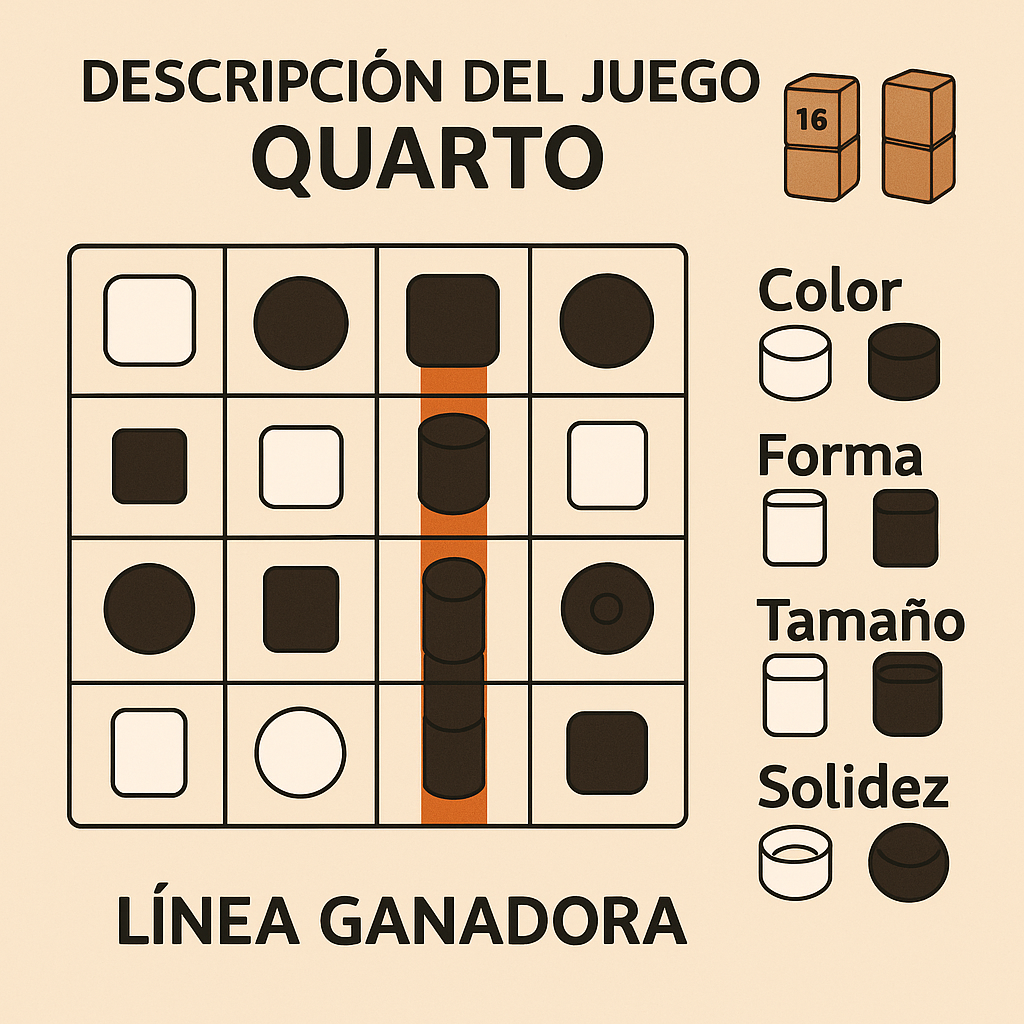
\includegraphics[width=0.48\textwidth]{quarto_tablero.png}
	\caption{Resumen visual del juego Quarto: tablero 4x4, piezas con atributos binarios, y condición de victoria.}
	\label{fig:quarto}
\end{figure}


Así, por ejemplo, puede haber una pieza \textit{blanca, alta, cuadrada y hueca} y otra \textit{negra, baja, redonda y sólida}; todas las 16 combinaciones posibles aparecen exactamente una vez \cite{muller2009}. Al inicio, la bolsa contiene las 16 piezas, y el tablero está vacío.

Los jugadores alternan turnos con una dinámica de "corte y elige": en cada movimiento un jugador \textbf{elige} una pieza disponible y el oponente la \textbf{coloca} en cualquier casilla vacía \cite{santana2012}. Es decir, un turno consta de dos fases: primero se coloca la pieza que quedó "activa" del turno anterior, y luego se selecciona la siguiente pieza que el rival deberá colocar.

Gana el jugador que, al colocar una pieza, completa una línea (horizontal, vertical o diagonal) de cuatro piezas que compartan al menos un atributo. Si el tablero se llena sin que nadie logre esto, la partida termina en empate \cite{muller2009}.



La complejidad combinatoria del Quarto es muy elevada: se estima en torno a $(16!)^2 \approx 4.4 \times 10^{26}$ partidas posibles si se considerara el espacio completo sin podas \cite{santana2012}. Esta cifra incluye todas las secuencias de elección y colocación de piezas (sin contar simetrías), lo que hace inabarcable una búsqueda exhaustiva del espacio completo.



\section{Representación Simbólica}

La representación de la realidad para el agente se basa en un \textbf{modelo simbólico} que capture el estado del juego.



\begin{figure}[h!]
	\centering
	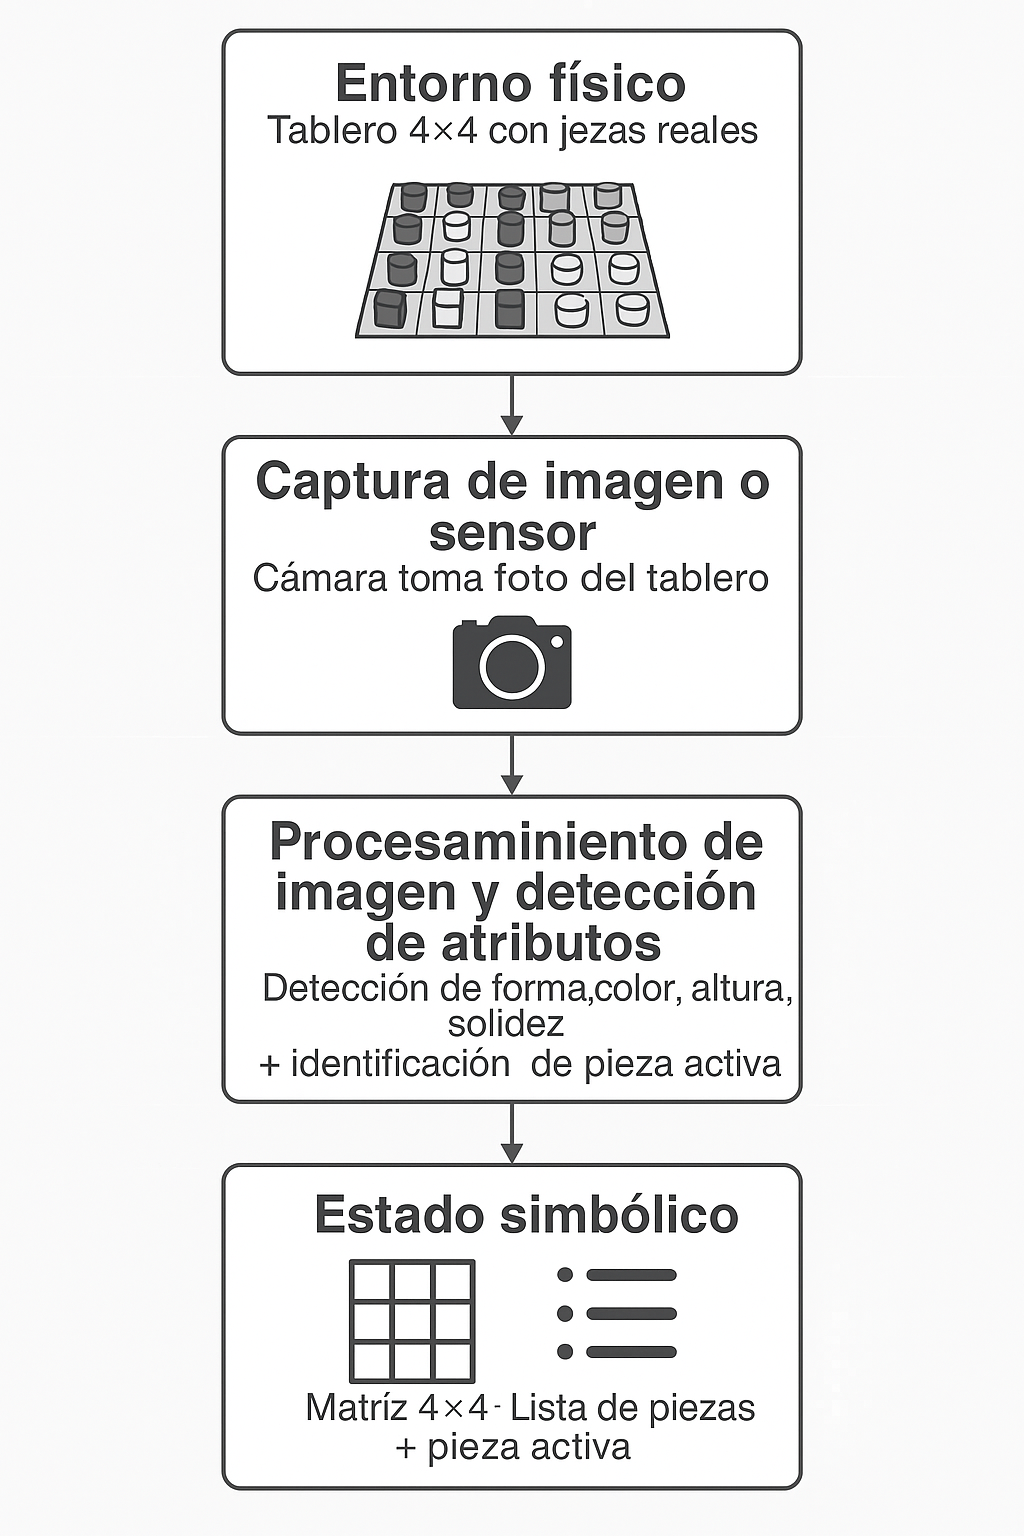
\includegraphics[width=0.95\linewidth]{img/representacion-realidad.png}
	\caption{Representación de la realidad para el agente inteligente en el juego Quarto. Se observa la secuencia: entorno físico, percepción mediante sensor, procesamiento de imagen, construcción del estado simbólico y ejecución de la acción física.}
	\label{fig:representacion_realidad}
\end{figure}

\subsection{Modelo de Tablero}
El tablero se representa como una matriz 4×4 de casillas. Cada casilla puede estar vacía o contener una pieza identificada por un código único (1–16).

\subsection{Codificación de Piezas}
Cada pieza se codifica como un vector de 4 bits (uno por cada atributo: color, tamaño, forma, solidez), o bien como un identificador de objeto que contenga esas propiedades. Los 16 identificadores (p. ej., P1, P2, …, P16) corresponden a las 16 combinaciones binarias posibles \cite{muller2009}.

\subsection{Estado de Juego}
El estado del juego incluye:
\begin{itemize}
\item Conjunto de 16 casillas con asignación (vacía o con pieza X)
\item Lista de piezas \textbf{disponibles} (las que aún no se han colocado)
\item Pieza "activa" que debe jugarse en el turno actual
\end{itemize}

\subsection{Percepción y Procesamiento}
El agente utiliza un sensor (por ejemplo, una cámara) para leer la disposición real de piezas en el tablero y su identificación. Mediante técnicas de visión por computador, el agente clasifica color y forma, y deduce el identificador de cada pieza física.





\section{Definición Ontológica}

La definición ontológica describe los elementos esenciales del dominio \textbf{Quarto}, sus relaciones y restricciones.

\subsection{Conceptos Principales}

\begin{itemize}
\item \textbf{Pieza}: Objeto con los atributos $\{\text{color}, \text{tamaño}, \text{forma}, \text{solidez}\}$. Cada combinación binaria es única.
\item \textbf{Casilla}: Posición del tablero identificada por coordenadas $(fila, columna)$ con valores del 1 al 4.
\item \textbf{Tablero}: Conjunto de 16 casillas organizadas en forma matricial 4×4.
\item \textbf{Jugador}: Actor que realiza alternadamente dos acciones: \textit{colocar} una pieza y \textit{elegir} la próxima pieza para el rival.
\item \textbf{Movimiento}: Asociación $\{pieza, casilla\}$ que resulta en colocar una pieza en una casilla vacía.
\item \textbf{Turno}: Ciclo de dos subacciones: colocar la pieza activa en el tablero y elegir la siguiente pieza para el oponente.
\end{itemize}

\subsection{Relaciones}

\begin{itemize}
\item \textbf{ocupa(pieza, casilla)}: Indica que cierta pieza está actualmente en esa casilla.
\item \textbf{disponible(pieza)}: Indica que la pieza aún no ha sido colocada en ninguna casilla.
\item \textbf{vacia(casilla)}: Indica que la casilla no está ocupada.
\item \textbf{pieza-activa(pieza)}: Identifica la pieza que debe colocarse en el turno actual.
\end{itemize}


\begin{figure}[h!]
	\centering
	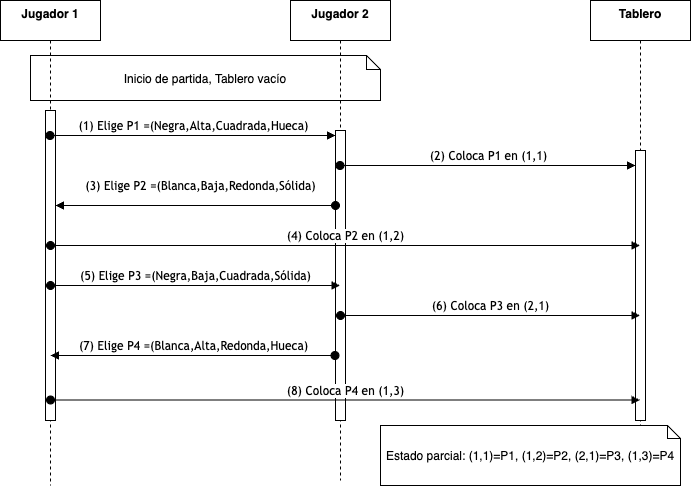
\includegraphics[width=0.95\linewidth]{img/diagrama-secuencia.png}
	\caption{Diagrama de secuencia para las primeras jugadas del juego Quarto entre Jugador 1 y Jugador 2. Se observa la interacción de elección y colocación de piezas en el tablero, con estado parcial al finalizar.}
	\label{fig:secuencia_quarto}
\end{figure}


\subsection{Restricciones del Dominio}

\begin{itemize}
\item Cada \textbf{Pieza} solo puede ser "disponible" o "ocupa" una única casilla, nunca dos.
\item Una \textbf{Casilla} solo puede contener a lo sumo una pieza.
\item No puede haber dos piezas idénticas en el juego (las 16 combinaciones son disjuntas).
\item Al finalizar un turno, \texttt{pieza-activa} cambia a otra pieza que el jugador elige para el rival.
\item \textbf{Condición de victoria}: existe al menos una línea de cuatro casillas contiguas (horizontal, vertical o diagonal) que contengan piezas con un atributo binario idéntico \cite{muller2009}.
\end{itemize}

\section{Diseño del Agente de Búsqueda}

El agente inteligente se estructura en tres bloques principales: \textbf{Percepción}, \textbf{Razonamiento (Búsqueda Adversarial)} y \textbf{Acción}.


\begin{figure}[h!]
	\centering
	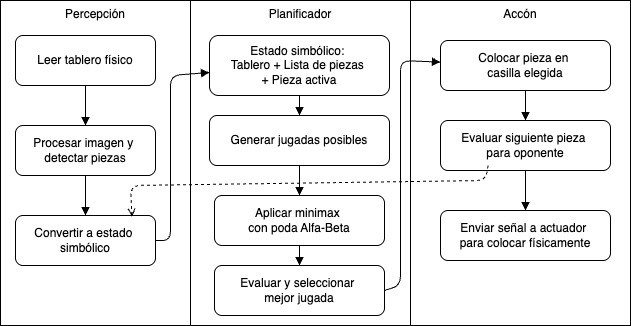
\includegraphics[width=0.95\linewidth]{img/diagrama-busqueda.png}
	\caption{Diagrama de flujo del agente inteligente para el juego Quarto, estructurado en tres fases: Percepción, Planificación y Acción. Se detalla el ciclo de lectura del entorno físico, razonamiento con poda Alfa-Beta y ejecución de acciones físicas.}
	\label{fig:diagrama_busqueda}
\end{figure}

\subsection{Percepción del Estado}

\begin{enumerate}
\item \textbf{Leer tablero físico}: Capturar imagen o leer sensor que detecta las 16 casillas.
\item \textbf{Procesar imagen y detectar piezas}: Clasificar cada casilla como "vacía" o "ocupada" y, si está ocupada, identificar atributos para asignar el código de pieza correcto \cite{muller2009}.
\item \textbf{Convertir a estado simbólico}: Actualizar la matriz 4×4 y la lista de piezas no jugadas.
\end{enumerate}

\subsection{Generación de Jugadas Posibles}

Dado el estado simbólico y la \textit{pieza activa}, el agente obtiene todas las casillas vacías. Cada casilla vacía $c$ genera una jugada candidata $(pieza\_activa, c)$.

\subsection{Algoritmo Minimax con Poda Alfa-Beta}

\subsubsection{Función de Evaluación Heurística}
\begin{itemize}
\item Si un movimiento conduce a una condición definitiva de victoria para el agente, asignar valor $+\infty$.
\item Si permite al oponente ganar inmediatamente, asignar valor $-\infty$.
\item Para estados no terminales, usar una heurística basada en el número de líneas de 3 piezas con posibilidad de completarse.
\end{itemize}

La heurística se define como:
\begin{equation}
h(s) = W_{\text{agente}}(s) - W_{\text{oponente}}(s)
\end{equation}

donde $W$ suma puntajes parciales de líneas de 3 piezas con atributos compartidos \cite{santana2012}.

\subsubsection{Expansión del Árbol de Juego}
\begin{itemize}
\item El estado inicial se expande generando nodos hijos para cada jugada $(pieza\_activa, casilla)$.
\item Para cada hijo, se determina la nueva pieza activa que el adversario recibirá.
\item El árbol crece alternando capas "colocación" y "elección de pieza".
\item Se podan ramas cuyo valor máximo/mínimo no influirá en la decisión final \cite{russell2016}.
\end{itemize}

\subsection{Selección de Pieza para el Oponente}



Después de colocar la pieza en la mejor casilla, el agente debe seleccionar la siguiente pieza que dará al rival:


\begin{enumerate}
\item \textbf{Evaluar cada pieza restante}: Para cada pieza $p$ en la lista de disponibles, simular que el oponente la coloca en las mejores casillas posibles para él.
\item \textbf{Escoger pieza "segura"}: Entre las piezas que no permiten victoria inmediata al rival, seleccionar la que minimice las oportunidades futuras del oponente \cite{santana2012}.
\item \textbf{Asignar pieza activa}: La pieza seleccionada se marca como la nueva pieza activa para el oponente.
\end{enumerate}


\begin{figure}[h!]
	\centering
	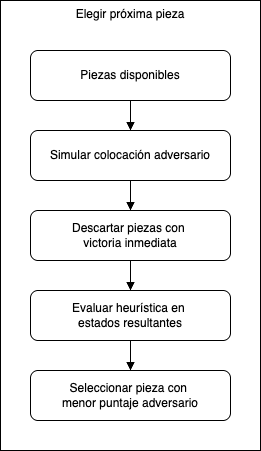
\includegraphics[width=0.95\linewidth]{img/asignar-pieza.png}
	\caption{Subproceso para seleccionar la próxima pieza.}
	\label{fig:asignar_pieza}
\end{figure}

\subsection{Ejecución Física de la Acción}

Una vez decidida la jugada $(pieza\_activa, casilla\_sel)$, se envía la orden al actuador (brazo robótico o interfaz gráfica) para colocar la pieza en la casilla. A continuación, se actualiza la lista de piezas disponibles y la pieza activa pasa a ser el identificador $p_{sel}$ que se dio al oponente.

\section{Conclusiones}

Se ha presentado un marco completo para el desarrollo de un agente inteligente para el juego Quarto, incluyendo una representación ontológica detallada del dominio y un diseño de arquitectura basado en búsqueda adversarial. La implementación del algoritmo minimax con poda Alfa-Beta, junto con funciones heurísticas específicas, permite al agente tomar decisiones estratégicas eficientes en tiempo real.

La complejidad combinatoria del Quarto requiere el uso de técnicas de poda y limitación de profundidad para hacer viable la búsqueda en el espacio de estados. El enfoque propuesto integra exitosamente la percepción del estado físico del juego con el razonamiento simbólico y la ejecución de acciones.

\begin{thebibliography}{9}

\bibitem{muller2009}
B. Müller, \textit{Quarto – Análisis del juego y estrategias de búsqueda}. Barcelona: Ediciones Gigamic, 2009.

\bibitem{russell2016}
S. J. Russell and P. Norvig, \textit{Artificial Intelligence: A Modern Approach}, 3rd ed. Pearson, 2016.

\bibitem{santana2012}
J. Santana and M. López, "Algoritmos adversariales para juegos de mesa: Aplicación en Quarto," \textit{Revista Iberoamericana de Inteligencia Artificial}, vol. 14, no. 2, pp. 45–58, 2012.

\end{thebibliography}

\end{document}